\chapter{Designing and modeling the system}\label{ch:designing_and_modeling}
This chapter includes the UPPAAL models in conjunction with corresponding UML
diagrams describing the implementation done in Ada. The UPPAAL models are used
for the validation and verification of the system that it meets the real-time
requirements set on the system. The connection from the UPPAAL models to the
UML diagrams presented here are to show that the implementation corresponds as
close as possible to the models verified.

For presentation purposes only the messages concerning basic functionality
during component and service discovery is presented in this chapter. After the
initial discovery and configuration process have been done the system continue
in normal operation mode with an extra set of SPA message types. Detailed
sequence diagrams over the component and service discovery process is shown in
section \ref{sec:discovery_process}.

\section{First iteration}
The first UPPAAL models were created after designing the basic structure of the
system. Each application will do the same thing which is receive, handle
and send messages. The difference between the applications is which
messages each application understands and which messages the application will
ignore. A processing node will at most have one CAS, one SM-L and one LS
but can have any number of applications running next to them. This inspired the
first iteration of UPPAAL models that the application automaton should be
possible to instantiate multiple times in UPPAAL but the other more specific
models can be used only ones. The basic component overview is shown in figure
\ref{fig:processing_node_overview} which is what the UPPAAL model is to
resemble as close as possible.

\begin{figure}[h]
    \centering
    
\includegraphics[width=\textwidth]{figures/processing_node_overview}
    \caption{A Processing Node overview with core SPA parts.}
    \label{fig:processing_node_overview}
\end{figure}

\subsubsection{A basic application}
The basic functionality of an application is that it should be able to identify
itself on the network, share its capabilities and request information from
other applications. An application is only connected to one subnet at a time.
The limitied functionality of an application makes for a basic two-layered
design where the upper-layer alter its behaviour depending on incoming
message types and the lower layer is only responsible for sending and receiving
messages on its subnet. The application sends out Local\_Hello message during
boot-up and receives a Local\_Ack response, all messages are modeled as
transition between different states. It then receives a logical address with
the Assign\_Address message. As final step it receives a Probe\_Request from
the Lookup Service to share its capabilities. Figure
\ref{fig:iteration1_application} shows the UPPAAL model.

\begin{figure}[h]
    \centering
    \includegraphics[width=\textwidth]{figures/iteration1_application}
    \caption{UPPAAL model of a first iteration application.}
    \label{fig:iteration1_application}
\end{figure}

\subsubsection{Central Addressing Service (CAS)}
Specifics for the CAS is that it assigns an address to itself so no need for
processing of Assign\_Address messages. As addition to basic application
functionality the CAS sends out address block to the requesting subnet
managers. Figure \ref{fig:iteration1_cas} shows the UPPAAL model.

\begin{figure}[h]
    \centering
    \includegraphics[width=\textwidth]{figures/iteration1_cas}
    \caption{UPPAAL model of a first iteration CAS.}
    \label{fig:iteration1_cas}
\end{figure}

\subsubsection{Lookup Service (LS)}
The additions the LS brings in is the processing of Request\_LS\_Probe,
Probe\_Reply and Probe\_Request messages, for service discovery purposes.
Figure \ref{fig:iteration1_ls} shows the UPPAAL model.

\begin{figure}[h]
    \centering
    \includegraphics[width=\textwidth]{figures/iteration1_ls}
    \caption{UPPAAL model of a first iteration LS.}
    \label{fig:iteration1_ls}
\end{figure}

\subsubsection{Local Subnet Manager (SM-L)}
In contrast to the other components the Subnet Manager manages most of the
interaction done in the subnet. It's responsible for answering all Local\_Hello
messages during component discovery and replying with an acknowledgement as
well as with an logical address assignment. As a last step it tells the LS to
send out Probe\_Requests to all active components on the subnet. Figure
\ref{fig:iteration1_sm_l} shows the UPPAAL model.

\begin{figure}[h]
    \centering
    \includegraphics[width=\textwidth]{figures/iteration1_sm_l}
    \caption{UPPAAL model of a first iteration SM-L.}
    \label{fig:iteration1_sm_l}
\end{figure}


\subsubsection{First iteration conclusions}
The CAS, LS and SM-L have specific functionality so they can only be used ones
when setting up a complete network of automata. The application model can be
instantiated multiple times as was the goal. At this level of abstraction
everything looks fine though the main goal with the UPPAAL model is to be able
to verify that the system behaves as aspected and can't reach unknown states or
deadlock. As the first iteration of models only shows the boot-up process it
will eventually reach deadlock when everything is set up. This is a drawback
as it doesn't relate very well with the actual design of the system, after
boot-up. This calls for another iteration and improvement of the different
UPPAAL automata.

Before heading to the second iteration it's time to take a closer look at the
UPPAAL automata and see what other parts need improvements, as it should
resemble the actual system as much as possible.

First of is the current automata use transitions to model sent and
received messages directly between the different automata. When a transition is
taken to send a message the receiving automaton takes a corresponding
transition to receive the message at the same time. This is in contrast with the
implementation where all messages go through a queue. The second iteration of
UPPAAL models should be modeled with proper queues that can be scaled in size.

The models only work with a set of eight different message types and in the
current design of the UPPAAL automata it is hard to add more types of messages.
The second iteration should make it possible to add and remove
specific message types with ease.

\section{Second iteration}
To improve the UPPAAL models a more detailed design is required of the system.
From the first iteration it's clear that the basic application can be designed
in a generic fashion. The CAS and LS is more specific instantiations of the
basic application and the SM-L has substantial differences. For easier
maintanence of the models during the second iteration it would be valuable if
the UPPAAL models could created in a modular way. Two main models would be the
"basic application" and the "SM-L".

Figure \ref{fig:iteration2_uml_component_overview} shows the component overview
after the second iteration. The design of the interfaces between the components
makes it easy to interchange which message types each "running task"
(application) can handle and how it communicates. A simple application that is
only connected to one subnet does not need the Routing component. The Routing
component is specifically created for the SM-L to be able to route traffic
within its own subnet and to other subnet managers over other types of subnets.

\begin{figure}[h]
    \centering
    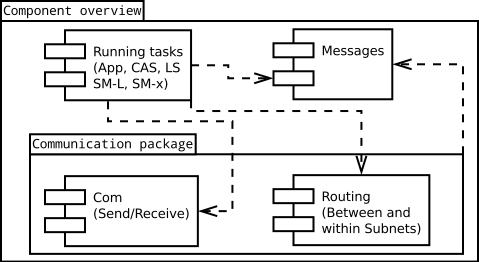
\includegraphics[width=\textwidth]{figures/iteration2_uml_component_overview}
    \caption{Component overview of a basic SPA implementation}
    \label{fig:iteration2_uml_component_overview}
\end{figure}

The design of the Communication package make use of the "Composite
pattern" where Routing objects and Com objects all inherit from the same
interface and where the Routing objects are of composite types. Figure
\ref{fig:iteration2_difference} shows the difference between a simple
application and the SM-L. The use of the composite pattern makes it possible
for a "Running task" in the application layer to easily swap out how it
connects to one or multiple networks.

\begin{figure}[h]
    \begin{subfigure}[b]{0.5\linewidth}
        \centering
            \includegraphics[width=0.9\textwidth]{figures/iteration2_uml_basic_application}
            \caption{An application}
            \label{fig:iteration2_uml_basic_application}
            \end{subfigure}%
        \begin{subfigure}[b]{.5\linewidth}
            \centering
            \includegraphics[width=0.9\textwidth]{figures/iteration2_uml_sm_l}
            \caption{A Subnet Manager}
            \label{fig:iteration2_uml_sm_l}
        \end{subfigure}
    \caption{The difference between a simple application and the SM-L.}
\label{fig:iteration2_difference}
\end{figure}

\subsubsection{The queues}
In the implementation of a Local SPA Subnet communication is done through
protected objects in Ada. Each protected objects includes two queues, one from
the application to the SM-L and one to the application from the SM-L. To model
this in UPPAAL the C-like language could be used to create the actual queues in
the background of the queue automaton. The finished queue is shown in figure
\ref{fig:iteration3_queue}. Each queue instantiated for each application
including the CAS and the LS.

\begin{figure}[h]
    \centering
    \includegraphics[width=\textwidth]{figures/iteration3_queue}
    \caption{Iteration 2 - The queue automaton}
    \label{fig:iteration3_queue}
\end{figure}

\subsubsection{A basic application}
\begin{figure}[h]
    \centering
    \includegraphics[width=\textwidth]{figures/iteration2_app}
    \caption{Iteration 2 - The application automaton}
    \label{fig:iteration2_app}
\end{figure}

After modeling the queues the application was up next. The application
automaton is shown in figure \ref{fig:iteration2_app}. In addition to the
queues implemented in UPPAAL C-like language a "Message" struct was also
defined to model a SPA message, including its header. Each message is modelled
with a from and a to address as well as an opcode identifying what type of
message it is.

A key assumption during iteration two was that upon receiving a message each
application should send a response immidietly. This was modelled in all
automata including the one for the applications. Upon receiving a message with
the opcode "Assign\_Address" or "Probe\_Request" another message was sent in
response before taking any other action. This introduced deadlock scenarios if
the queue back to the SM-L was full the automaton for the application could not
take any transition and if the queue to the application was full as well both
the SM-L and the application would be waiting for each other to empty their
respective incoming queue.

A solution to this that was tested. The solution allowed each application to
throw away all incoming messages if no response could be sent back out. In turn
each application had to keep track of which messages it had sent out
and which responses it expected. After a few improvements this solution turned
out to be too complex, resulting in a model that was hard to understand and
time consuming to verify.

\subsubsection{Second iteration conclusions}
As too many problems arose with iteration two only the application and queue
automata are shown. Even though the end result of iteration two was not good
enough improvements was made throughout the model.

\begin{itemize}
    \item Iteration two added the queue automaton which made it possible to
        model if and how the size of the queues would effect the system.
    \item The addition of the Message struct made it possible to model
        different type of messages being sent in the system without much
        trouble.
    \item The logic throughout the system was vastly improved.
    \item The possiblity to vary the number of applications was kept.
\end{itemize}

\section{Third iteration}
The main focus of the third iteration was to remove the possibility of
deadlocks. The underlying cause of deadlock was the tight coupling between
receiving a message and sending a response. To losen up the coupling different
approaches could be taken. One solution was to add time contraints such that if
the outgoing queue was full the automata would wait for a set amount of time
and then retry. It was early on apparent that this wouldn't improve the
deadlock situation.

A second solution and the one chosen was to make the assumption that when
receiving a message the information is stored locally and then the application
return to its idle state. From the idle state the application can then make a
choice whether to receive another message or send a new message. The tight
coupling was by this change completly removed.

The third and final iteration automata are shown in the following images and
together with the Queue automaton (Fig. \ref{fig:iteration3_app}) from
iteration two they form the final model of a SPA Local Subnet that use Ada
Protected Objects as communication channel.

\begin{figure}[ht]
    \centering
    \includegraphics[width=\textwidth]{figures/iteration3_app}
    \caption{Iteration 3 - The application automaton}
    \label{fig:iteration3_app}
\end{figure}

\begin{figure}[ht]
    \centering
    \includegraphics[width=\textwidth]{figures/iteration3_sm_l_receive_loop}
    \caption{Iteration 3 - The receive loop parts of the SM-L automaton}
    \label{fig:iteration3_iteration3_sm_l_receive_loop}
\end{figure}

\begin{figure}[ht]
    \centering
    \includegraphics[width=\textwidth]{figures/iteration3_sm_l_send_loop}
    \caption{Iteration 3 - The send loop parts of the SM-L automaton}
    \label{fig:iteration3_iteration3_sm_l_send_loop}
\end{figure}

\begin{figure}[ht]
    \centering
    \includegraphics[width=\textwidth]{figures/iteration3_sm_l_route_loop}
    \caption{Iteration 3 - The routing loop parts of the SM-L automaton. All
    messages with a destination that is not the SM-L are routed through this
    loop after first being received in the "Receive loop".}
    \label{fig:iteration3_iteration3_sm_l_route_loop}
\end{figure}

\begin{figure}[ht]
    \centering
    \includegraphics[width=\textwidth]{figures/iteration3_cas}
    \caption{Iteration 3 - The Central Addressing Service automaton}
    \label{fig:iteration3_cas}
\end{figure}

\begin{figure}[ht]
    \centering
    \includegraphics[width=\textwidth]{figures/iteration3_ls}
    \caption{Iteration 3 - The Lookup Service automaton}
    \label{fig:iteration3_ls}
\end{figure}

% \section{An event-triggered alternative}
% TODO: All models and comments about an event-triggered alternative.

\pagebreak
\section{Verification}
To verify that the system is free of deadlocks and livelocks the following
UPPAAL verification queries were used. As the automata only test the component
and service discovery process the goal is to reach a deadlock state in the end.
To verify that it is only the final deadlock that can be reached the queries
verify that all automata are in Idle states and the appropiate variables have
been set (all applications have been properly registered in the network).

The livelock query make sure that all paths eventually reach the final deadlock
state.

\subsubsection{Verification query for deadlocks}
\lstset{language=C}
\begin{lstlisting}[frame=single]
A[] deadlock imply
    CAS.Idle && SM_L.Idle && LS.Idle &&
    LS.Received_Probe_Reply[CAS_Address] == true &&
    forall(Application_ID: Application_ID_Type)
        Application(Application_ID).
            Local_Ack_Received == true &&
        Application(Application_ID).
            Assign_Address_Received == true &&
        Application(Application_ID).Idle &&
        LS.Received_Probe_Reply[Application_ID] == true
\end{lstlisting}

\subsubsection{Verification query for livelocks}
\lstset{language=C}
\begin{lstlisting}[frame=single]
A<> CAS.Idle && SM_L.Idle && LS.Idle &&
    LS.Received_Probe_Reply[CAS_Address] == true &&
    forall(Application_ID: Application_ID_Type)
        Application(Application_ID).
            Local_Ack_Received == true &&
        Application(Application_ID).
            Assign_Address_Received == true &&
        Application(Application_ID).Idle &&
        LS.Received_Probe_Reply[Application_ID] == true
\end{lstlisting}
